\chapter{Background Theory}
\label{chp:theory} 


\section{Modern Robotics}

\section{Modelling and Simulation}

\subsection{Some Terminology}

\subsubsection{Coordinate Systems and Poses}

Coordinate systems are essential in the field of robotics. 

\subsection{Robot Modelling}

\subsection{Simulating in Gazebo}

\section{ROS}

\subsection{Introduction}

Roots of the \ac{ROS} can be traced back to Stanford University at the beginning of the 2000s. At Stanford, several robotics software frameworks, including \ac{STAIR} and the \ac{PR} program, were created to provide dynamic, flexible and well tested foundations for further robot development and research. In 2007, a nearby start-up company and robot incubator, Willow Garage, sought to build upon these concepts, and initiated a collaborative and open development process of a new software framework, which eventually became \ac{ROS}. This framework can be used under the BSD open-source license, which means that ... Today, \ac{ROS} comes in many forms and comprise hundreds of advanced packages, algorithms and drivers, making it applicable for hobbyists, industrial automation and everything in between. 

\subsection{Important ROS Concepts}

The following descriptions are included in order to provide a complete, self-contained description of the project implementation. Similar descriptions can be found on the official \ac{ROS} website (INSERT LINK HERE), as well as in any book on \ac{ROS} (see \cite{A BOOK ON ROS}). 

\subsection{Structure of a ROS Application}

\section{Software}

\subsection{Qt}

\subsection{PCL}

\section{The Kinect Sensor}

\section{Software Tools}

\subsection{Point Cloud Library}

\subsection{ROS}

\subsection{Qt}


\subsection{Current Research and Applications}

\section{Modern Sensors in Autonomous Robots}

\subsection{Depth Cameras}

\subsubsection{Different Methods for Depth Perception}

In the context of this thesis, a depth camera is considered to be a sensor which the functionality of a regular video camera 

A depth camera can be described as a regular color video camera with the ability to create spatial images. In the context of this thesis, a depth camera can  more precisely be described as a RGB-D camera, which is short for red, green, blue and depth camera. A regular RGB camera will project a spatial scene onto a rectangular pixel grid, where each pixel contains intensity values for red, green and blue colors. These pixel values represents the detected scene. A major problem with RGB cameras is the significant loss of information. The information loss is mostly a consequence of 3d to 2d projection and digital quantization. RGB-D cameras have the means to reduce this information loss by mapping the pixel values to spatial coordinates, turning each pixel into voxels and the image into a point cloud of voxels. 

Different variations of depth cameras will usually fall into one of two categories: active or passive. Passive sensors perceive the surroundings as it is, without actively interfering with the environment as a part of the sensing process. A typical passive RGB-D sensor is the stereo camera. Stereo cameras use a stream of synchronized image pairs to perceive depth. The image pairs are displaced along the horizontal axis, and the depth information is extracted by searching for mutual information in the image pairs. How far the information is displaced from the left to the right image is directly related to how far away from the camera the information source is located. 

Active sensors depend on some form of projection onto the surroundings. For depth cameras, the projection is usually in the form of laser or infra red light. In RGB-D cameras it is essential that the projected light is distinguishable from the visible spectrum. The Kinect sensor used in this project is an example of an active RGB-D sensor. A proper introduction to the Kinect, will follow shortly.

\subsubsection{Natural User Interfaces}

Forslag:
When a group of designers are developing a new \ac{GUI}, they will often use a conceptual model when planning their design. The conceptual model is the mental model the designers want to put into the head of the user. All users will develop their own individual mental model, which is their high level understanding of how the \ac{GUI} works. A conceptual model may contain metaphors for things  the user already is familiar with. A painting program for example may use a metaphor for a canvas, paint brushes and palettes. When the mouse icon changes to a paint brush, most users will have an intuitive understanding of what it can do and how it is used. A \ac{NUI} will seek to remove the metaphors and create a more seamless interaction between the user and the machine. Some \ac{NUI}s may allow a user to write text with a pen instead of a keyboard, or dictate a letter with their voice while the computer converts audio into text. 

Forslag:
The idea behind a \ac{NUI} is to make \ac{HMI} as seamless and natural as possible. A \ac{NUI} allows the user to communicate without tools such as a keyboard or a mouse. Initially starting as ideas and rare research projects, \ac{NUI}s can now be considered to have become ubiquitous, where the most common form is the touch screen found in smart phones and tablets. 

The Microsoft Kinect sensor was initially designed as a \ac{NUI} for the Xbox 360 gaming console. The sensor allows users to use gestures and sounds to play console games. Later on, Microsoft has released SDKs, enabling developers to create \ac{NUI} applications for for Windows. 

The modern RGB-D sensors which are commonly used in robot research projects today were initially intended as \ac{NUI}.

\subsubsection{Kinect for Xbox 360}

Kinect for Xbox 360 is the RGB-D sensor used in this project. The device was initially intended as a \ac{NUI} for gaming and 

The depth sensor 

\begin{figure}[p]
    \centering
    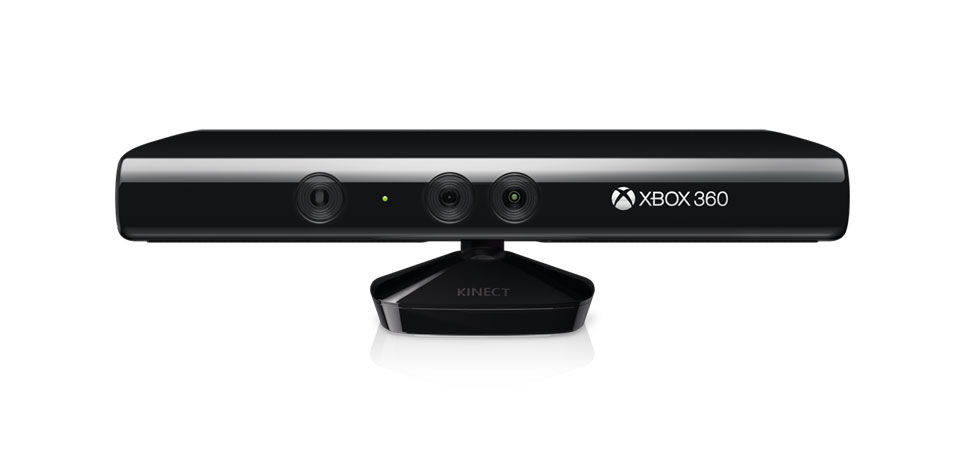
\includegraphics[width=0.8\textwidth]{kinect360}
    \caption{Awesome Image}
    \label{fig:kinect360}
\end{figure}

\begin{figure}[p]
    \centering
    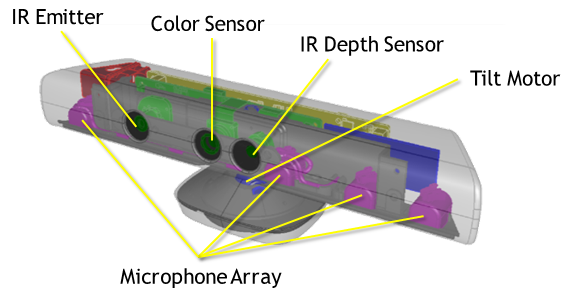
\includegraphics[width=0.8\textwidth]{kinect360_exp}
    \caption{Awesome Image}
    \label{fig:kinect360_exp}
\end{figure}


\subsection{Laser Scanners (LIDAR)}

\subsection{Odometers}

\subsection{Sensor Fusion}


\section{RTAB-Map}